\chapter{World of Warcraft (WoW) Features in MIA} \label{WoW}
\pagestyle{fancy}

\section{WoW Fishbot} \label{WoWFishbot}

\begin{note}
	As of World of Warcraft (WoW) version 7.2, this fishbot is fully functional.
\end{note}

The World of Warcraft (WoW) fishbot implementation within MIA was created solely for educational purposes. This fishbot violates the terms of use of WoW and should only be used at your own risk. The fishbot is designed to simulate fishing for ones character in WoW. 

\subsection{Setup and Configuration}

Before running the fishbot, there are a few things that need to be properly configured, otherwise the bot will either not work or not work efficiently. First, one must disable the hardware cursor in the system settings. This can be done by pressing escape, system, advanced, then setting hardware cursor to disable (see figure \ref{hardwar cursor}). Be sure to click apply before closing out of the settings.

\begin{lstlisting}
ESC > System > Advanced > Hardware Cursor > DISABLE > Apply
\end{lstlisting}

\begin{figure}[h]
	\centering
	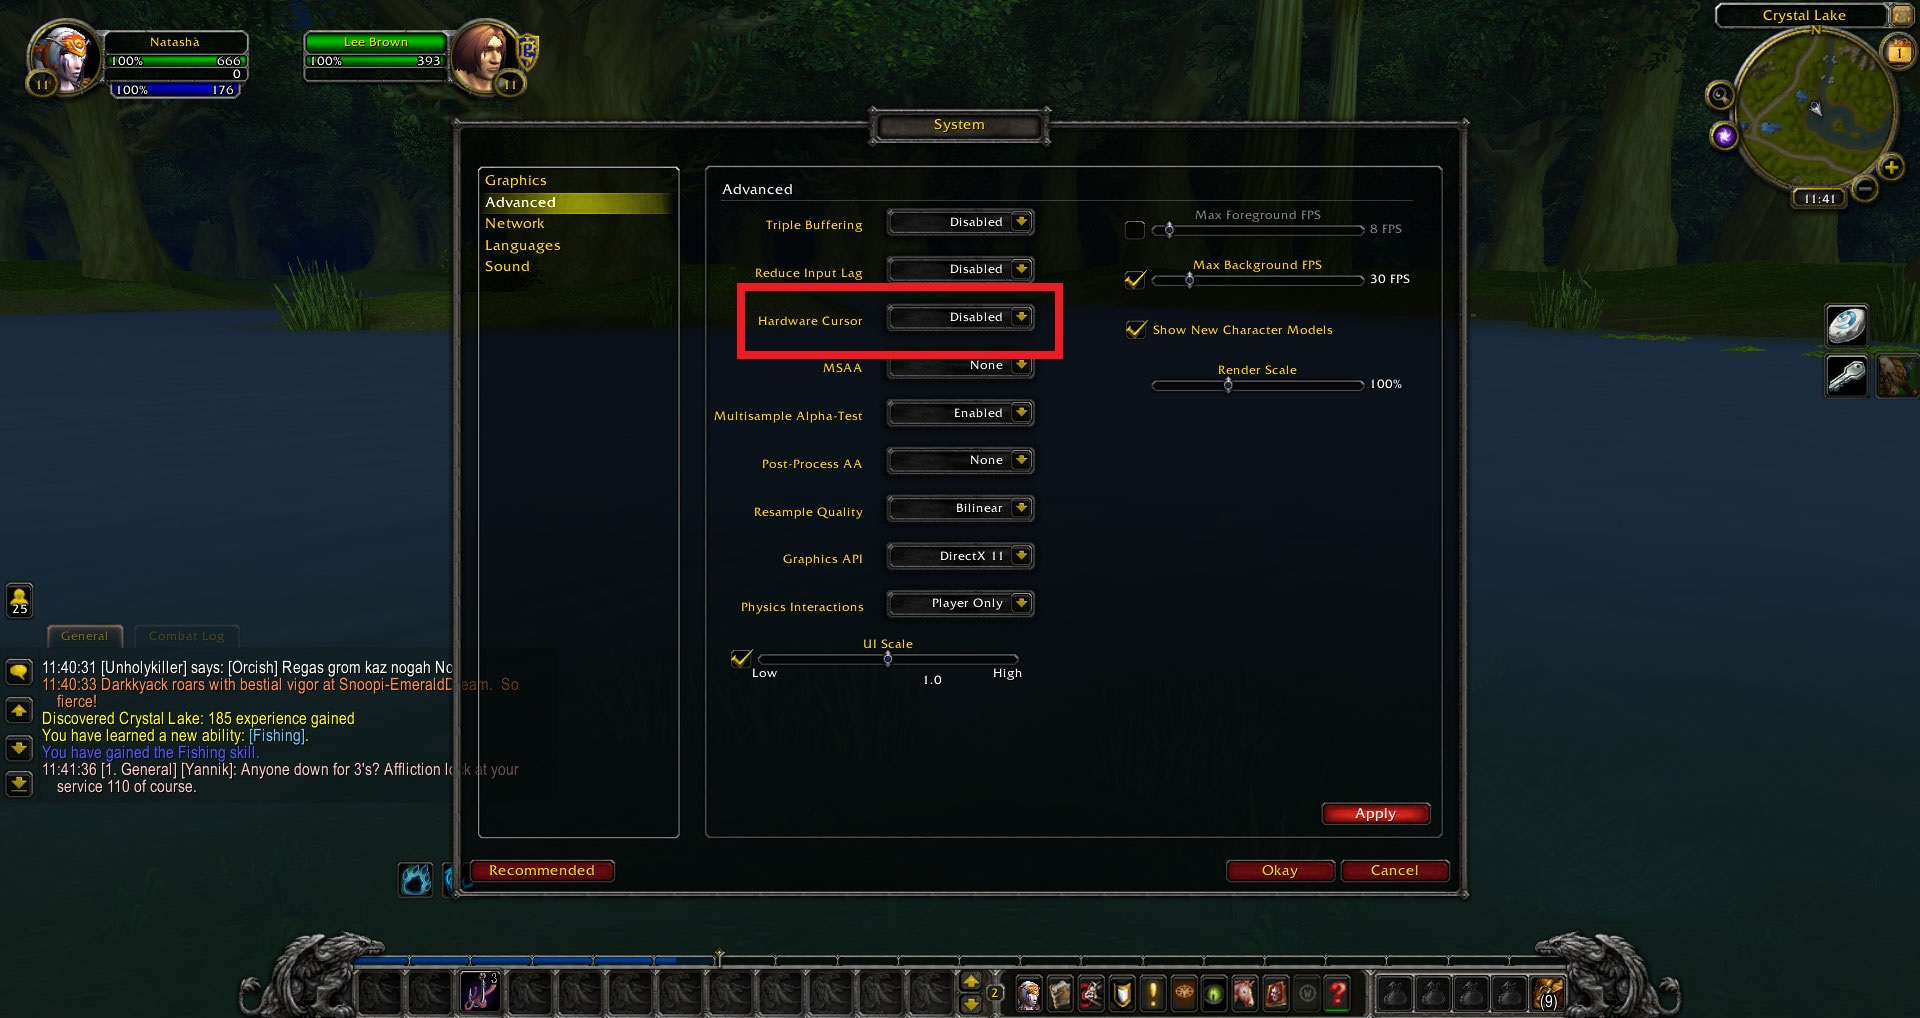
\includegraphics[width=0.9\textwidth]{Images/WoWScrnShot_040118_234154.jpg}
	\caption{Visual representation of the location of the option for disabling the hardware cursor. In order for the WoW fishbot to work, this option must be disabled.} \label{hardwar cursor}
\end{figure}

After disabling the hardware cursor, the coordinates for cast locations need to be set. It is recommended that the user zoom into first person when using the fishbot though this is not required for functionality. First, place the cast button on the action bar (see figure \ref{cast bar}). By default, the fishbot uses button 3 for cast, but upon running the fishbot the user will be prompted to change the settings. Similarly, a lure can be added to the bar, which by default is placed in action bar slot 8. A lure is optional and the fishbot program will ask if one is being used upon runtime.

\begin{figure}[h]
	\centering
	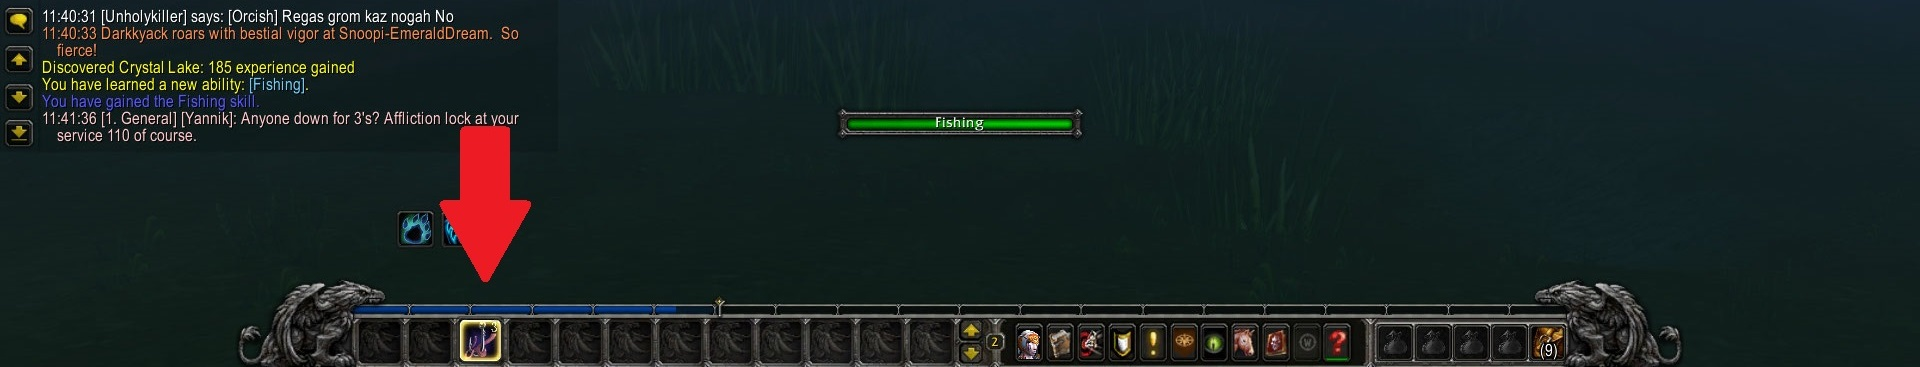
\includegraphics[width=0.9\textwidth]{Images/WoWScrnShot_040118_234212.jpg}
	\caption{Visual representation of the location of the cast option on the action bar.} \label{cast bar}
\end{figure}

The MIAC contains four separate variables that will most likely need to be configured for each user for use with the fishbot. The default values were set based on the creators environment and are not guaranteed to work for everyone. The options and their default values (at the time of writing this) are listed below.

\begin{lstlisting}
# Variables relating to the fishbot implementation inside MIA.
WoWFishBotStartX=725
WoWFishBotStartY=360
WoWFishBotEndX=1230
WoWFishBotEndY=495
\end{lstlisting}

These values, \inlinecode{WoWFishBotStartX, WoWFishBotStartY, WoWFishBotEndX, WoWFishBotEndY}, define the area that the fishbot will search for the fish bobber within. The first two parameters, \inlinecode{WoWFishBotStartX, WoWFishBotStartY} define the coordinates of the point A in figure \ref{fishbot square}. The second two parameters, \inlinecode{WoWFishBotEndX, WoWFishBotEndY} define the coordinates of the point B in figure \ref{fishbot square}. The MIA fishbot will search this area for the bobber during operation. The best method to determine the proper coordinates to use is to spam the cast option and observe the area that the bobber lands. The suggested coordinates for A and B are near where they are located in figure \ref{fishbot square}, however any coordinates can be used. To determine the proper coordinates, one can use the \inlinecode{find mouse} command in MIA which will determine the coordinates at the location of ones cursor.

After these parameters are set, the fishbot can be run in MIA by using the \inlinecode{fishbot} command. There are a few other variables and parameters that can be set by the user but the others are optional. These other optional parameters that are contained in the MIAC are as follows.

\begin{lstlisting}
# Variables relating to the fishbot implementation inside MIA.
WoWFishBotIncrement=40
WoWFishBotNumOfCasts=10000
WoWFishBotDelay=10000
\end{lstlisting}

First, the \inlinecode{WoWFishBotIncrement} variable defines the step size that the MIA program will search for the bobber by. This can be seen in figure \label{fishbot increments}. A smaller step size will cause the fishbot to find the bobber slower but more accurate, whereas a faster step size will cause a faster search but is less accurate. The default value for this is 40, but should be decreased if the bobber is missed by the fishbot. The next parameter, \inlinecode{WoWFishBotNumOfCasts} is how many times the fishbot will cast before ending it's program. This can be whatever the user desires. 

\begin{figure}[h]
	\centering
	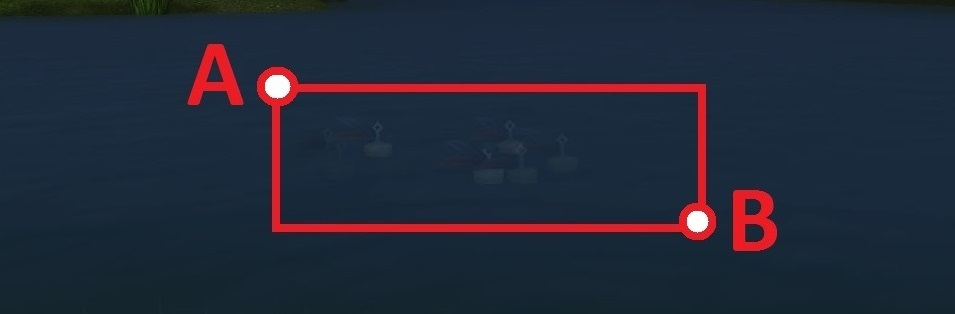
\includegraphics[width=0.9\textwidth]{Images/WoWScrnShot_040118_234212b.jpg}
	\caption{The red square represents the region in which the casted bobber lands. The two points labeled A and B are positions that one would want to set as the proper coordinates in the MIAC (see section \ref{MIAC} for more details).} \label{fishbot square}
\end{figure}

\begin{figure}[h]
	\centering
	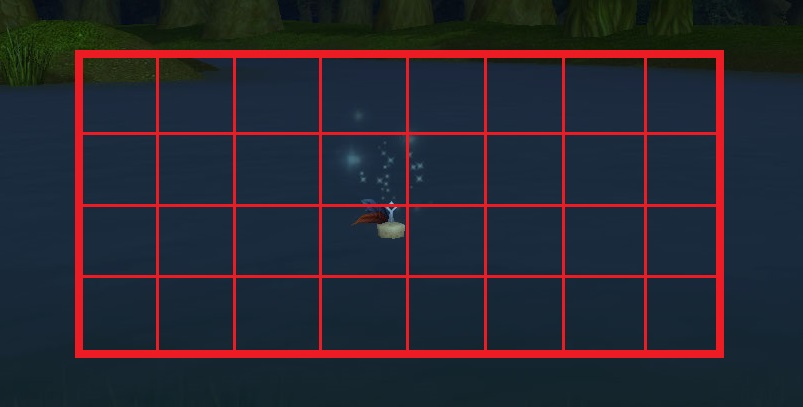
\includegraphics[width=0.9\textwidth]{Images/WoWScrnShot_040118_234227b.jpg}
	\caption{The red square similar to that shown in figure \ref{fishbot square} partitioned into squares of size defined by the \inlinecode{WoWFishBotIncrement} value.} \label{fishbot increments}
\end{figure}

The last parameter, \inlinecode{WoWFishBotDelay} is what defines how fish are caught. The MIA fishbot catches fish by chance. There is a plan to improve the method to catch fish by, but for now the program waits a specific number of milliseconds after finding the bobber before clicking it. Thus, there is a certain probability that a fish is caught. By default this value is 10000ms.

\section{Mailbox Management} \label{WoWMailbox}

Section in development.